%Correct the file name.
%X: book number
%Y: part number
%ZZZ: page number in three digits. So page 3 would be 003.

\documentclass[11pt]{amsbook}

\usepackage{../HBSuerDemir}	% ------------------------
\usepackage{mathtools}
\usepackage{amsmath}
\begin{document}

% ++++++++++++++++++++++++++++++++++++++
\hPage{b1p2/333}
% ++++++++++++++++++++++++++++++++++++++




% =======================================
\[
    \xi = \rho(\cos\psi+ i\: \sin\psi)
\]
is an nth root of the complex number
\[
    z = r (\cos\theta + i\: \sin\theta),
\]
it satisfies the equation \:\:  $\xi^n = z$  \:\: which, by the use of
\\De Moivre's formula, gives 
\[
    \rho^n(\cos\:n\psi+i\:\sin\:n\psi=\:r\:\cos(\theta\:+\:2k\pi)\:+\:i\:\sin(\theta\:+\:2k\pi)   
\]
and there

\[
    \rho^n\:=\:r,\enspace  n\psi\:\theta\:+\:2k\pi
\]
\[
    \rho=\sqrt[n]{r},\enspace \psi = \frac{\theta}{n} \:+\:k\frac{2\pi}{n}\:,\enspace k\in  \mathbb{Z}.
\]
\\Hence z has n distinct roots given by
\[
    z_{k} = \sqrt[n]{r} \Big( \cos(\frac{\theta}{n} \:+\:k\:\frac{2\pi}{n})\:+\:i\:\sin(\frac{\theta}{n} \:+\:k\:\frac{2\pi}{n}) \Big) , \:k=1,\:2,\:\dots \: ,\:n.
\]

    Since $\: \mid z_{k} \mid \:=\:\sqrt[n]{r},\:$ all these roots $\:\:z_{1},\:z_{2},\:\dots\:z_{n},\:$ lie
\\on the circle with center at the origin and radius  $\sqrt[n]{r}$  as \\vertices of a regular n-gon.

In particular, the nth roots of l (unity) are 
\[
    \varepsilon_{k} \: = \: \cos\:k\:\frac{2\pi}{n} \:+\:i\:\sin\: k\:\frac{2\pi}{n} \:,\: \:k=1,\:2,\:\dots \: ,\:n.
\]
one of which, namely $\varepsilon_{n}$,  is the
\\number l (Note that  $\varepsilon_{n}\:=\:\varepsilon_{0}$).

If one of the nth roots is of z is $z_{1}$, then all the nth 
\\roots of z are obtained multipling $z_{1}$ by $\varepsilon_{1}\:,\:\dots\:,\:\varepsilon_{n}.$

The roots of the polynomial equation $z^n\:-\:1\:=\:0$ being
\\$\varepsilon_{1}\:,\:\dots\:,\:\varepsilon_{n}$, the following properties are the consequences of
\\the relations between the roots and coefficients:


\begin{align*}
    \sigma_{1} 
        &= \sum \varepsilon_{k}
         = \varepsilon_{1} + \dots +\varepsilon{n}
         =0\\
    \sigma_{2} 
        &= \sum_{k<l}\varepsilon_{k}\varepsilon_{l}
         =\:\varepsilon_{1}\varepsilon_{2}\:+\dots+\varepsilon_{1}\varepsilon_{n}\:+\dots+\varepsilon_{n-1}\varepsilon_{n}
         =\:0\\
    \sigma_{3} 
        &=\:\sum_{k<l<m}\varepsilon_{k}\varepsilon_{l}\varepsilon_{m}\:
         =\:0\\
    &\vdots\\
    \sigma_{n-1}
        &=\:0.
\end{align*}

%=======================================================
\end{document}  

%==== templates ====

%==== environments ====

%\begin{figure}[htb]
%	\centering
%	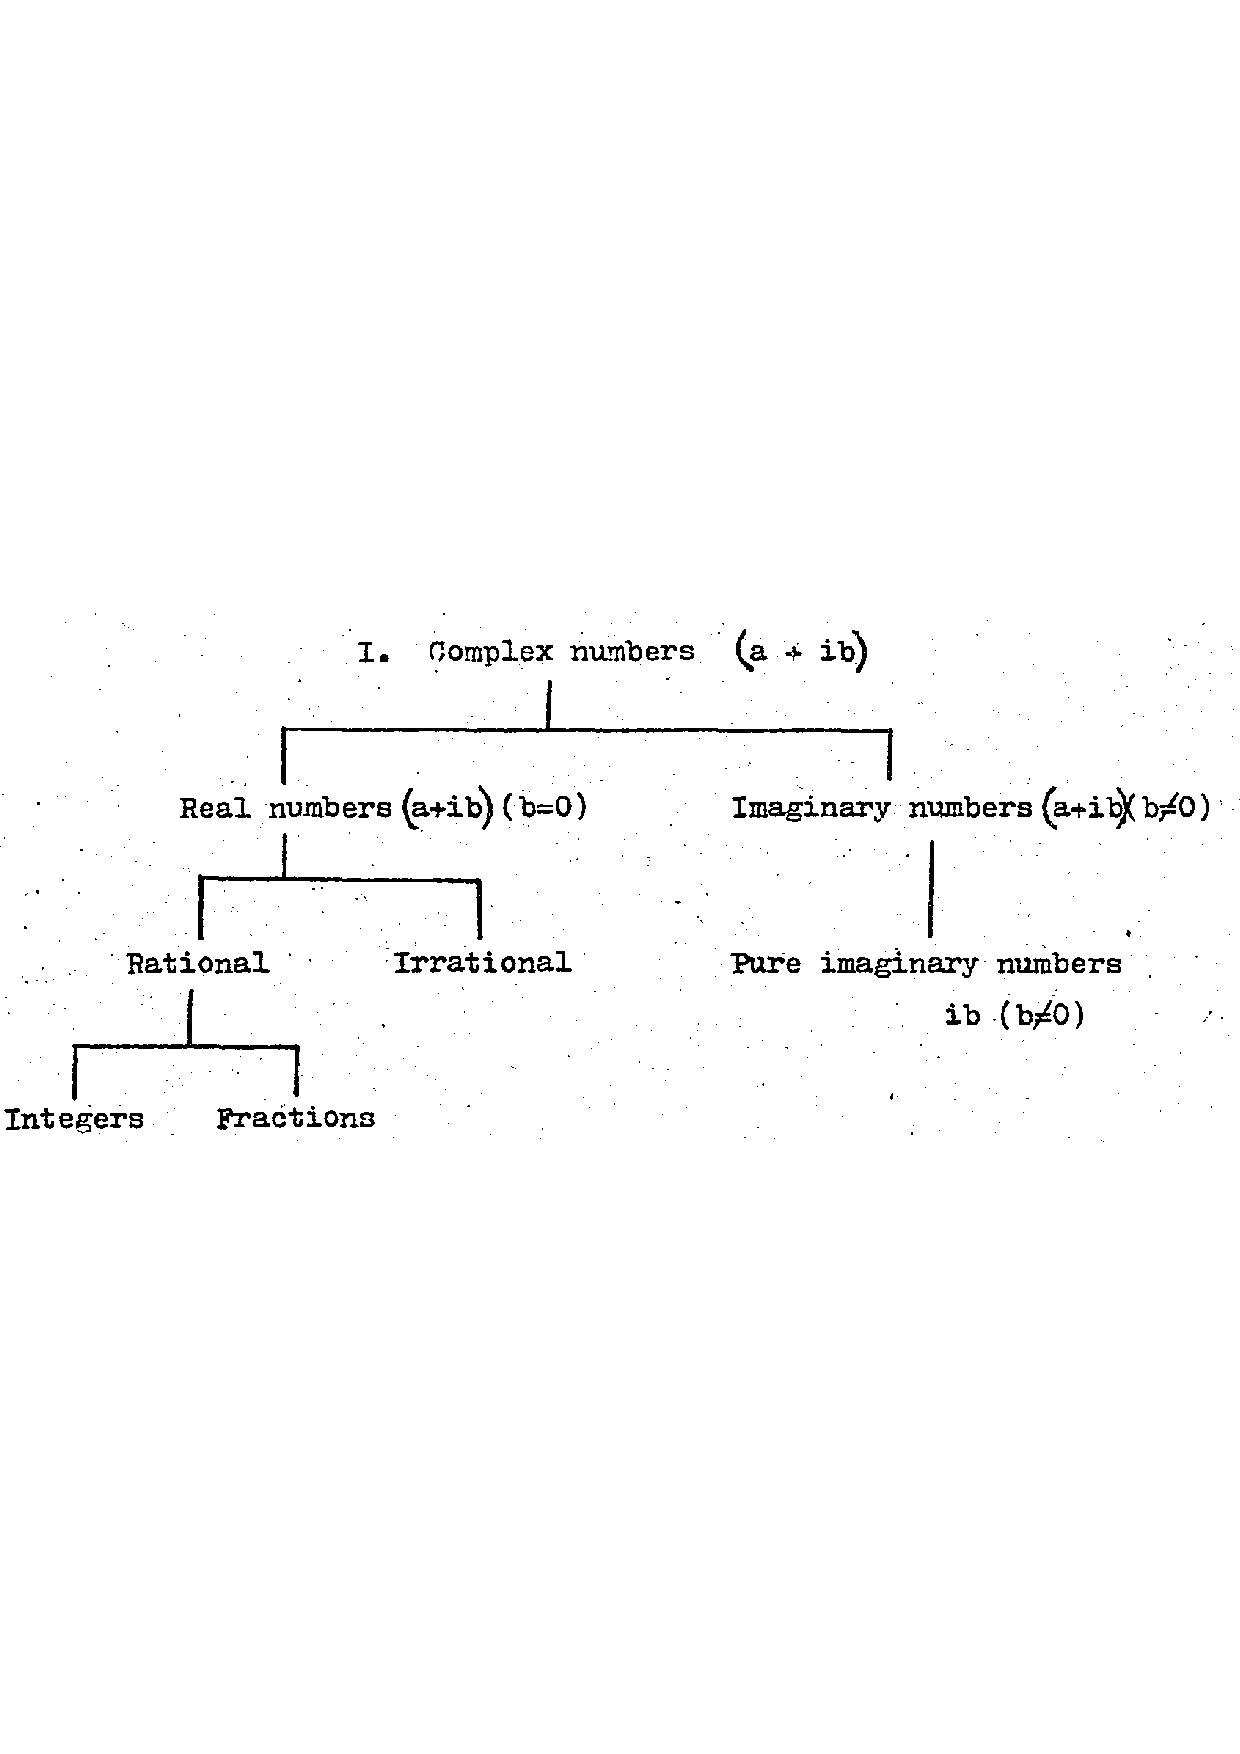
\includegraphics[width=0.9\textwidth]{images/SD-1-1p15A}
%	\caption{Classification of complex numbers}
%	\label{fig:classificationOfComplexNumbersA}
%\end{figure}

%\begin{center}
%\begin{tabular}{cc}
%\end{tabular}
%\end{center}

%\begin{exmp}
%\begin{hSolution}
%\end{hSolution}
%\end{exmp}

%\begin{hEnumerateAlpha}
%\end{hEnumerateAlpha}

%\begin{hEnumerateRoman}
%\end{hEnumerateRoman}

%$
%\begin{bmatrix}
%\end{bmatrix}
%$

%\frac{aaaa}{bbb}
%\frac{a_{n}}{b_{n}}
%\left( aaaa \right)
%\Longrightarrow

%\begin{multicols}{2}
%	bb
%\columnbreak
%	aa
%\end{multicols}
